\addcontentsline{toc}{chapter}{LAMPIRAN}
\chapter*{Lampiran Pertama}
\label{app:pertama}
\addcontentsline{loa}{chapter}{\protect\numberline{A}Lampiran Pertama}
%-----------------------------------------------------------------------
% Konten lampiran di sini, misalnya:
%------------------------------------------------------------------------
Lampiran dalam bentuk berisi
\begin{enumerate}[noitemsep]
	\item  Manual Penggunaan aplikasi
	\item Copy Surat Pengantar Survey/pengambilan data dan surat keterangan hasil uji cobatempat penelitian
	\item Instrumen pengujian atau pengambilan data (misal : kuesioner) 
\end{enumerate}


\chapter*{KETENTUAN PENULISAN LAPORAN TUGAS AKHIR }
\label{app:kedua}
\addcontentsline{loa}{chapter}{\protect\numberline{B}Lampiran Kedua}
%------------------------------------------------------
% Konten lampiran kedua di sini.
%------------------------------------------------------
\section*{Penyajian Tabel }
Judul tabel ditulis secara singkat tetapi jelas, dan ditempatkan  di  atas  tabel, tanpa diakhiri dengan titik dan ditulis dengan tebal. Huruf pertama pada kata pertama judul ditulis kapital, kataselanjutnya dengan huruf kecil. Apabila judul tabel lebih dari satu baris maka harus ditulis satu spasi.Pada prinsipnya tabel tidak boleh dipenggal. Apabila tabel berukuran cukup besar maka, jika diperlukan, ukuran huruf dapat diperkecil tetapi harus tetap mudah terbaca. Apabila tabel terpaksa dipenggal, maka pada halaman lanjutan tabel dicantumkan nomor tabel dan ditulis kata (lanjutan) tanpa judul. Apabila tabel harus dibuat dalam bentuk horisontal (landscape), maka bagian atas tabel harus diletakkan di sebelah kiri. Jika tabel dikutip dari referensi maka sitasi dituliskan pada bagianterakhir judul. Perkecualian untuk tabel yang memodifikasi beberapa data yang berasal dari berbagai sumber, maka sitasi ditunjukkan dengan simbol pada data dan di bagian bawah tabel dituliskan referensi yang dimaksudkan. Contoh Tabel.
\begin{table}[h]
	\centering
	\caption{Daftar Tabel}
	\label{tab:daftar_tabel}
	\begin{tabular}{cp{8cm}c}
	\toprule
		\textbf{No} & \textbf{Judul Tabel} & \textbf{Halaman} \\
	\midrule
		1 & Tabel 1: Distribusi Data Penelitian & 10 \\

		2 & Tabel 2: Hasil Analisis Statistik & 15 \\
	
		3 & Tabel 3: Ringkasan Temuan & 20 \\
	\bottomrule
	\end{tabular}
\end{table}

\section*{Contoh Long Table}
Berikut adalah daftar tabel yang digunakan dalam penelitian ini:

\begin{longtable}{c p{8cm} c}
	\caption{Daftar Tabel Panjang} \label{tab:daftar_tabel_panjang} \\
	\toprule
	\textbf{No} & \textbf{Judul Tabel} & \textbf{Halaman} \\
	\midrule
	\endfirsthead % Akhir header halaman pertama
	
	\caption[]{(Lanjutan) Daftar Tabel Panjang} \\
	\toprule
	\textbf{No} & \textbf{Judul Tabel} & \textbf{Halaman} \\
	\midrule
	\endhead % Header untuk halaman berikutnya
	
	\midrule
	\multicolumn{3}{r}{\textit{Lanjutan di halaman berikutnya}} \\
	\endfoot % Footer untuk setiap halaman kecuali terakhir
	
	\bottomrule
	\endlastfoot % Footer untuk halaman terakhir

		1 & Tabel 1: Distribusi Data Penelitian & 10 \\
	2 & Tabel 2: Hasil Analisis Statistik & 15 \\
	3 & Tabel 3: Ringkasan Temuan & 20 \\
	4 & Tabel 4: Data Pendukung Awal & 25 \\
	5 & Tabel 5: Analisis Tambahan & 30 \\
	6 & Tabel 6: Evaluasi Kinerja & 35 \\
	7 & Tabel 7: Perbandingan Metode & 40 \\
	8 & Tabel 8: Kesimpulan Data & 45 \\
	9 & Tabel 9: Rekomendasi Penelitian & 50 \\
	10 & Tabel 10: Lampiran Data Tambahan & 55 \\
	11 & Tabel 11: Statistik Lanjutan & 60 \\
	12 & Tabel 12: Validasi Hasil & 65 \\
	13 & Tabel 13: Catatan Tambahan & 70 \\
	14 & Tabel 14: Ringkasan Akhir & 75 \\
	
		1 & Tabel 1: Distribusi Data Penelitian & 10 \\
	2 & Tabel 2: Hasil Analisis Statistik & 15 \\
	3 & Tabel 3: Ringkasan Temuan & 20 \\
	4 & Tabel 4: Data Pendukung Awal & 25 \\
	5 & Tabel 5: Analisis Tambahan & 30 \\
	6 & Tabel 6: Evaluasi Kinerja & 35 \\
	7 & Tabel 7: Perbandingan Metode & 40 \\
	8 & Tabel 8: Kesimpulan Data & 45 \\
	9 & Tabel 9: Rekomendasi Penelitian & 50 \\
	10 & Tabel 10: Lampiran Data Tambahan & 55 \\
	11 & Tabel 11: Statistik Lanjutan & 60 \\
	12 & Tabel 12: Validasi Hasil & 65 \\
	13 & Tabel 13: Catatan Tambahan & 70 \\
	14 & Tabel 14: Ringkasan Akhir & 75 \\
		1 & Tabel 1: Distribusi Data Penelitian & 10 \\
	2 & Tabel 2: Hasil Analisis Statistik & 15 \\
	3 & Tabel 3: Ringkasan Temuan & 20 \\
	4 & Tabel 4: Data Pendukung Awal & 25 \\
	5 & Tabel 5: Analisis Tambahan & 30 \\
	6 & Tabel 6: Evaluasi Kinerja & 35 \\
	7 & Tabel 7: Perbandingan Metode & 40 \\
	8 & Tabel 8: Kesimpulan Data & 45 \\
	9 & Tabel 9: Rekomendasi Penelitian & 50 \\
	10 & Tabel 10: Lampiran Data Tambahan & 55 \\
	11 & Tabel 11: Statistik Lanjutan & 60 \\
	12 & Tabel 12: Validasi Hasil & 65 \\
	13 & Tabel 13: Catatan Tambahan & 70 \\
	14 & Tabel 14: Ringkasan Akhir & 75 \\
		1 & Tabel 1: Distribusi Data Penelitian & 10 \\
	2 & Tabel 2: Hasil Analisis Statistik & 15 \\
	3 & Tabel 3: Ringkasan Temuan & 20 \\
	4 & Tabel 4: Data Pendukung Awal & 25 \\
	5 & Tabel 5: Analisis Tambahan & 30 \\
	6 & Tabel 6: Evaluasi Kinerja & 35 \\
	7 & Tabel 7: Perbandingan Metode & 40 \\
	8 & Tabel 8: Kesimpulan Data & 45 \\
	9 & Tabel 9: Rekomendasi Penelitian & 50 \\
	10 & Tabel 10: Lampiran Data Tambahan & 55 \\
	11 & Tabel 11: Statistik Lanjutan & 60 \\
	12 & Tabel 12: Validasi Hasil & 65 \\
	13 & Tabel 13: Catatan Tambahan & 70 \\
	14 & Tabel 14: Ringkasan Akhir & 75 \\
\end{longtable}

Referensi tabel dapat dilihat di \ref{tab:daftar_tabel_panjang}.

\section*{Penyajian Gambar }
Gambar dalam skripsi meliputi : bagan alir, grafik, peta, foto, dan diagram kerja. Penyajian gambar dalam penyusunan naskah skripsi mengikuti ketentuan berikut. Judul gambar diletakkan di bawah gambar, tanpa diakhiri dengan titik dan ditulis dengan huruf tebal. Huruf pertama pada kata pertama judul ditulis kapital, kata selanjutnya dengan huruf kecil. Apabila judul gambar lebih darisatu baris maka harus ditulis satu spasi. Keterangan gambar dituliskan pada tempat-tempat yang kosong di dalam gambar dan jangan pada halaman lain. Bila gambar disajikan melebar sepanjang tinggi kertas, maka bagian atas gambar diletakkan di sebelah kiri.
Untuk gambar yang terdiri dari beberapa bagian harus digunakan keterangan urutan menggunakan (a), (b), dan seterusnya, dengan keterangan yang tercakup pada bagian judul gambar. Seluruh gambar harus diatur pada satu halaman yang sama. Untuk gambar berwarna hendaknya dapat dicetak warna atau diatur dengan pewarnaan yang kontras.
Jika gambar dikutip dari referensi maka sitasi dituliskan pada bagian terakhir judul gambar.Untuk gambar yang dikutip dari internet, hendaknya diperhatikan resolusi dan ketajaman gambar. Untuk gambar yang berasal dari hasil scanning harap diperhatikan tingkat resolusi dan ketajaman gambar. Jika diperlukan, hasil scan dapat dilengkapi dengan teks tertentu. Penamaan gambar  ditulis dibagian bawah gambar letak center. Gambar~\ref{wsn}  Merupakan contoh gambar Tugu Jogja.
      \begin{figure}[H]
	\centering
	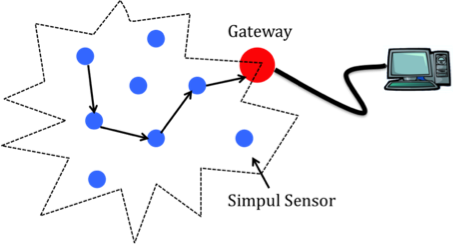
\includegraphics{gambar/wsn}
	\caption{Jaringan sensor nirkabel.}
	\label{wsn}
\end{figure}

 